\subsection{Modelo Fisico}
\subsubsection{Motor elegido}

\textbf{Microsoft Sql Server 2008}

\subsubsection{Diagrama fisico}
\subsubsection{Script de creacion de base de datos fisica}
	\begin{lstlisting}
		TODO: CREATE BBDD SCRIPT.
	\end{lstlisting}
\begin{landscape}
	\begin{figure}[t]
	  \centering	
		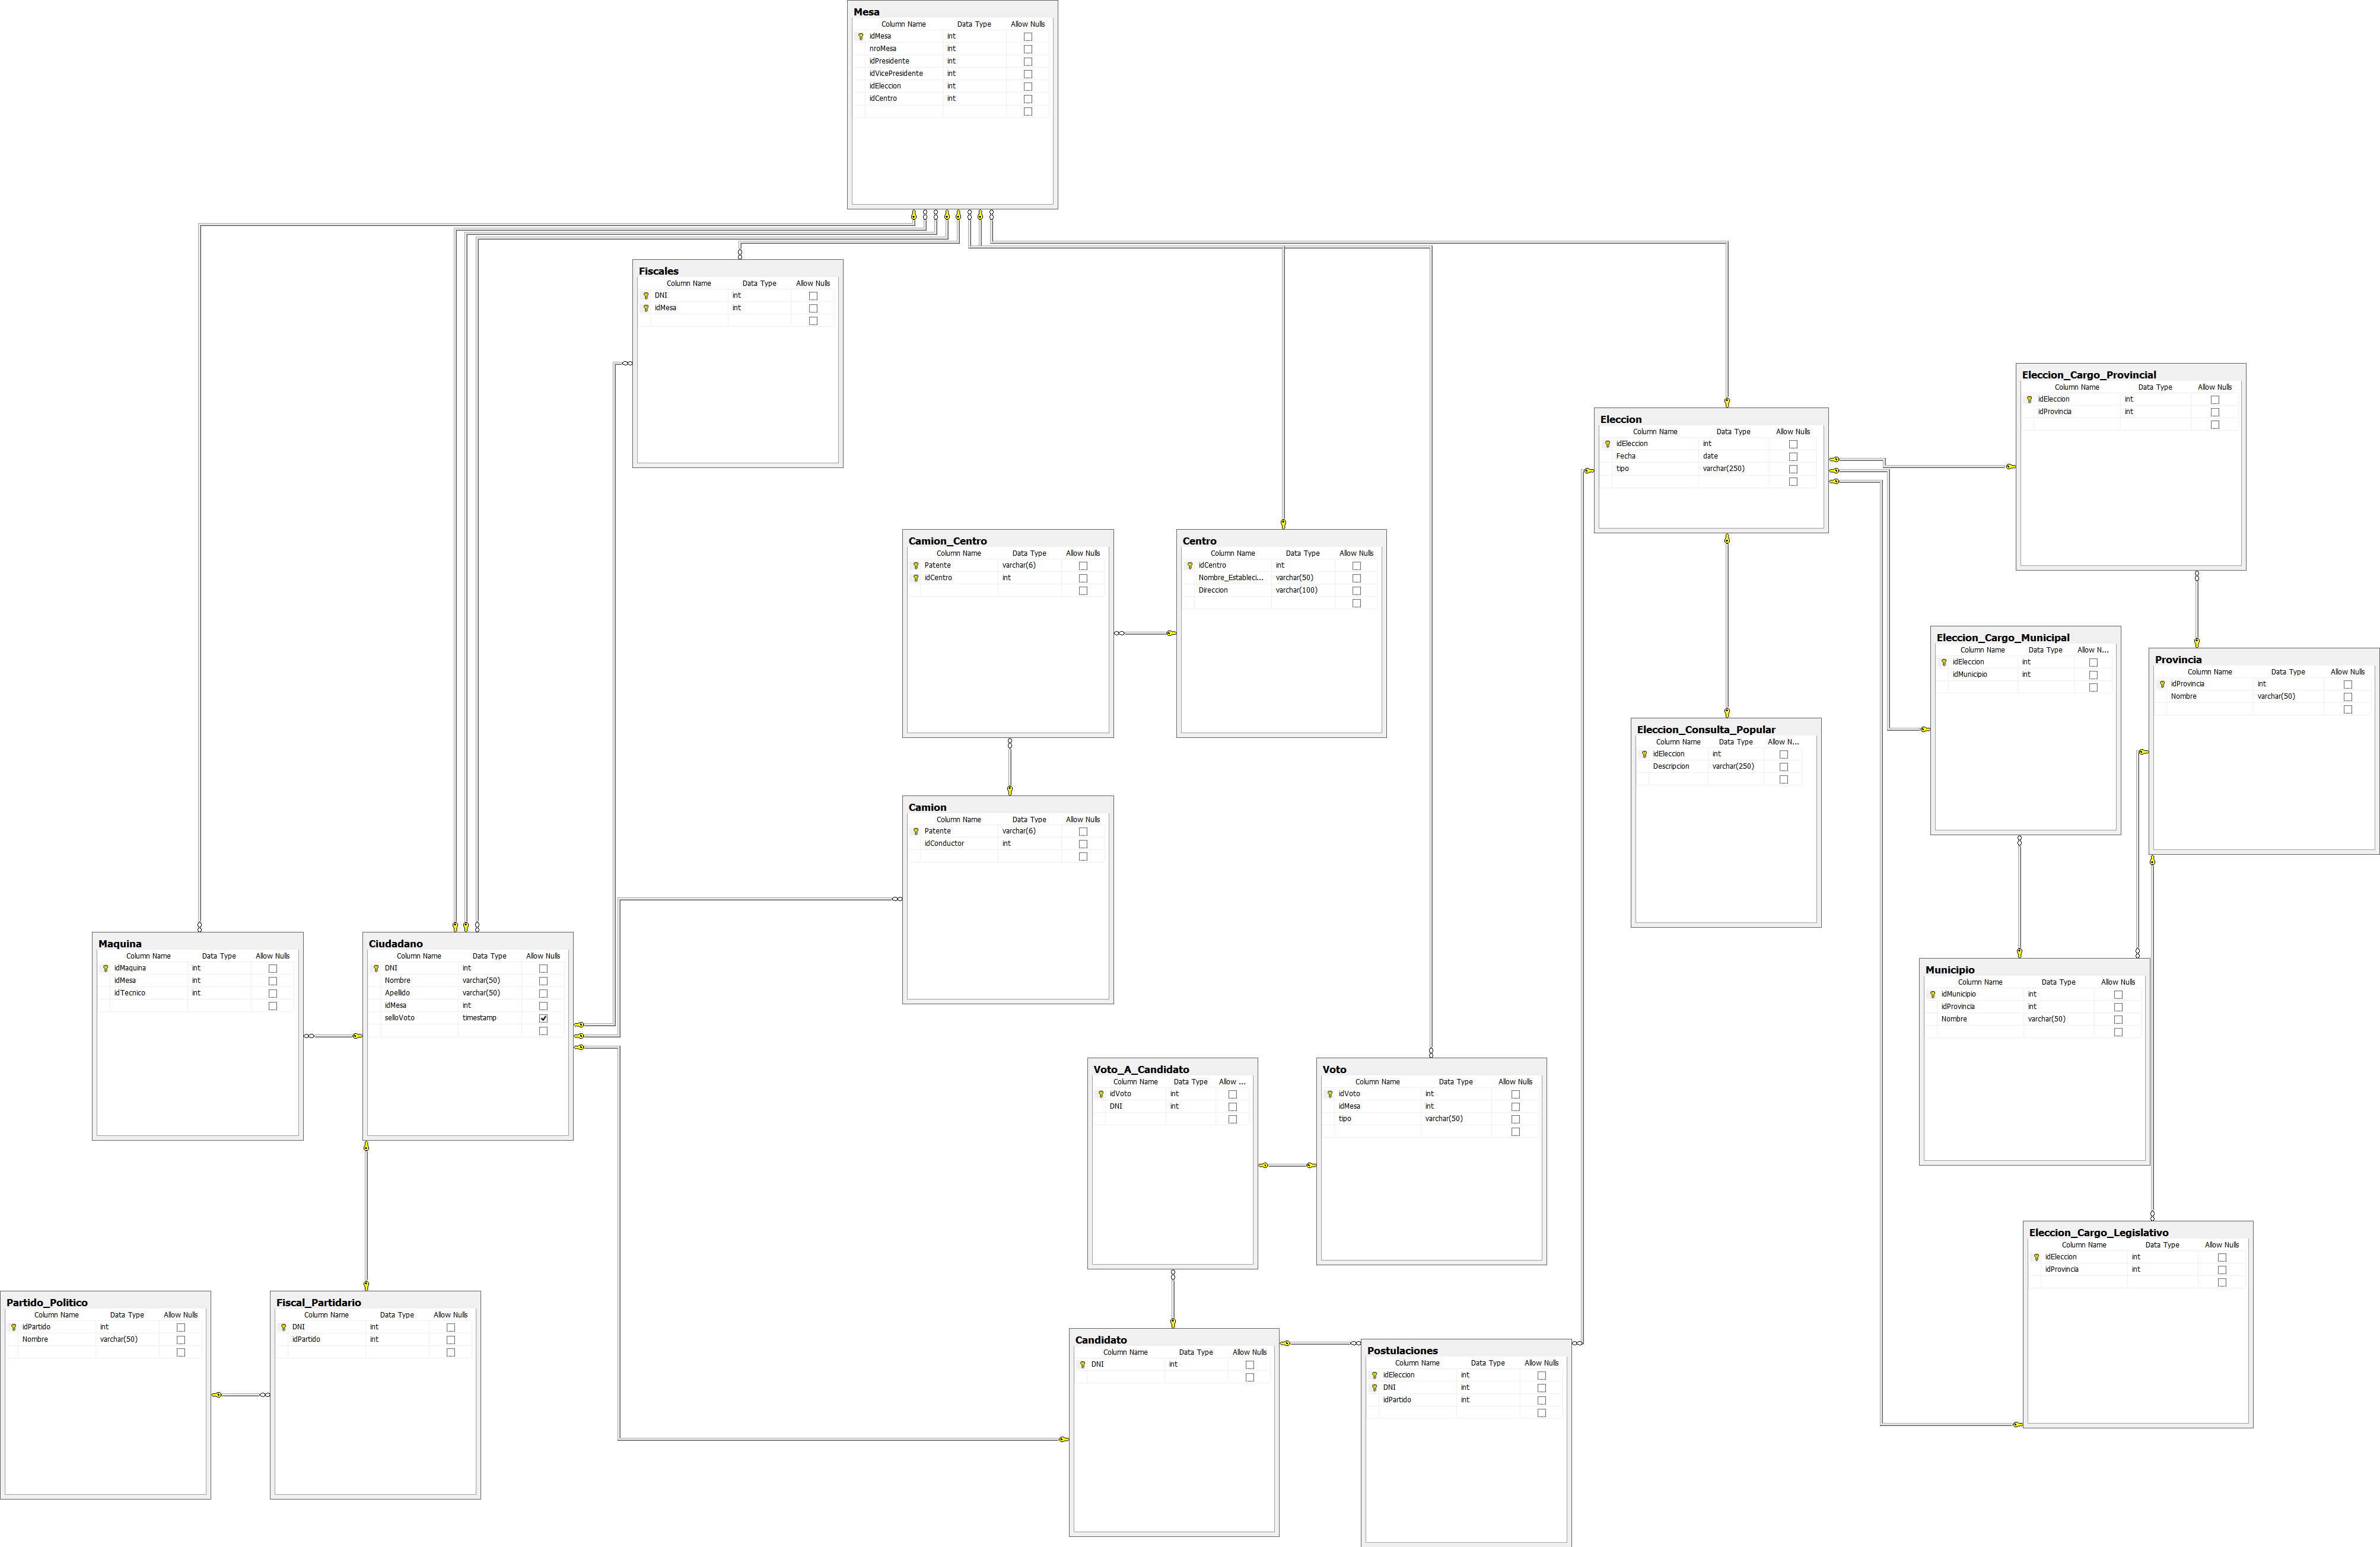
\includegraphics[scale=0.35]{fig/modelo-fisico.png}
	  \caption{Diagrama fisico.}
	\end{figure}
\end{landscape}
\subsubsection{Modelado fisico de las restricciones con triggers}
Modelaremos las restricciones al modelo utilizando funcionalidades provistas por el motor de la base de datos, como ser \textbf{Stored Procedures}, \textbf{Triggers}, \textbf{Checks}, etc. segun nos parezca conveniente. A continuacion se presenta el modelado de las restricciones.

\begin{itemize}
	\item Con respecto a las restricciones 1 y 2, referidas al voto y el sello en el padron, no podemos modelarlas con before y after triggers dado que no tenemos forma de navegar desde la tabla voto hacia el padron(no se guarda info de la persona en la tabla voto.). Con lo cual crearemos un stored procedure, que realizará la operacion de voto como una transacción, verificando que el sello sea NULO antes de insertar el voto y que el sello contenga el timestamp una vez insertado el voto. Tambien debe verificar que el voto sea a un candidato postulado para esa eleccion(la eleccion puede obtenerse de mesa), restriccion 7.
		\begin{itemize}
			\item Toda persona que vota en una mesa, debe tener nulo el campo selloVoto del padron para dicha mesa. ie. No permitir que la gente vote mas de una vez por eleccion.
			\item Para voto que se inserta se debe actualizar correctamente la fecha y hora en la que voto y poniendo el “sello” virtual en el padron asignando un valor no nulo a cuandoVoto.
			\item Un voto a candidato tiene que ser a un candidato que este postulado en esa eleccion.
		\end{itemize}

	\item Before insert trigger sobre tabla voto. navegamos a mesa y de mesa a eleccion y chequeamos que el campo tipo de la eleccion corresponda con el campo tipo del voto.
		\begin{itemize}
			\item Todos los votos para una eleccion son: o bien consulta popular o bien de tipo candidato según corresponda el tipo de eleccion
			\item Si la eleccion es una consulta popular, los votos deben ser si/no. Sino, deben ser candidatos
		\end{itemize}
		\begin{lstlisting}
			CREATE TRIGGER trg_check_selloVotoEsNull on Voto INSTEAD OF INSERT AS 
			BEGIN
				SET NOCOUNT ON
					INSERT INTO Voto(
						SELECT * FROM INSERTED
						WHERE 
						)
					blablabla, TODO
			END
		\end{lstlisting}
	
	\item{Queda implicada por el stored procedure de voto, que chequea sello null y marca no null el sello luego. No hay forma que de se inserten mas votos que personas}. \fk{Alguien piense esto a ver si no estoy flasheando plz.}
		\begin{itemize}
			\item La suma de los votos de todas las mesas de todos los candidatos debe ser menor o igual(votos en blanco diferencia) a la cantidad de ciudadanos que tiene el timestamp cuandoVoto? No nulo en el padron de dicha eleccion. (notar que esto tambien lo acota por la cantidad de ciudadanos). 
		\end{itemize}

	\item Queda determinado por la PK de la tabla Postulaciones.
		\begin{itemize}
			\item No hay candidatos repetidos en una eleccion.
		\end{itemize}

	\item Before insert trigger en postulaciones que no permita hacer insert si ya existe un candidato para dicho partido politico en dicha eleccion.
		\begin{itemize}
			\item Cada partido politico presenta un solo candidato.
		\end{itemize}
		\begin{lstlisting}
			CREATE TRIGGER trg_check_selloVotoEsNull on Postulaciones INSTEAD OF INSERT AS 
			BEGIN
				SET NOCOUNT ON
					INSERT INTO Postulaciones(
						SELECT * FROM INSERTED
						WHERE 
						)
					blablabla, TODO
			END
		\end{lstlisting}
	
	\item Before insert trigger en Mesa que verifique que en esa eleccion, no haya otras mesas donde este ciudadano sea tecnico, presidente, vicepresidente, fiscal o conductor
	\item Before insert trigger en Conductor que verifique que en esa eleccion, no haya  mesas donde este ciudadano sea tecnico, presidente, vicepresidente o fiscal.
		\begin{itemize}
			\item Un ciudadano no pueda ser tecnico, presidente, vicepresidente o fiscal en una misma eleccion.
			\item Un ciudadano no puede ser conductor y tecnico, presidente, vicepresidente o fiscal en una misma eleccion.
		\end{itemize}	

	\item Before insert trigger en Padron que verifique que para ese DNI, no exista otra mesa, de la misma eleccion, que ya lo tenga asociado.
		\begin{itemize}
			\item Un ciudadano vota en una sola mesa por eleccion.
		\end{itemize}

	\item Before insert en Mesa para ver que la maquina asignada no este asignada a otra mesa en esa eleccion.
		\begin{itemize}
			\item Una maquina funciona en una sola mesa por eleccion.
		\end{itemize}

\end{itemize}





\fk{OJO QUE VAMOS A USAR TRANSACCION EN UN STORED PROCEDURE.}
ojo con los insert triggers y los updates, habria que prohibir los updates o hacer triggers en insert y update?
no se deberian permitir deletes ni updates sobre voto(y posiblemente otras tablas). ??